\section{Software processes}
\subsection{Software specification}
\subsubsection{Requirements election and analysis}
\begin{itemize}
	\item Beobachtung des existierenden Systems
	\item Absprache mit Nutzern und Entwicklern
	\item Anforderungsanalyse
	\item Entwicklung von Modellen und Prototypen
\end{itemize}
\subsubsection{Requirements specification}
\begin{itemize}
	\item Anforderungen formulieren und dokumentieren
	\item Nuteranforderungen (abstrakt)
	\item Systemanforderungen (detailliert)
\end{itemize}
\subsubsection{Requirements validation}
\begin{itemize}
	\item Umsetzbarkeit
	\item Konsistenz
	\item Vollständigkeit
	\item Fehlerkorrektur 
\end{itemize}
\subsection{Software design and implementation}
\subsubsection{Architectural design}
\begin{itemize}
	\item Systemstruktur
	\item Hauptsächliche Strukturen und Beziehungen
	\item Vertrieb
\end{itemize}
\subsubsection{Database design}
\begin{itemize}
	\item Datenstrukturen
	\item Darstellung in Datenbanken
\end{itemize}
\subsubsection{Interface design}
\begin{itemize}
	\item Eindeutige Interface-Spezifikationen
	\item Kommunikation zwischen Komponenten, ohne Kenntnis der Implementation
\end{itemize}
\subsubsection{Component selection and design}
\begin{itemize}
	\item Suche nach wiederverwendbaren Komponenten
	\item Definiere Veränderungen bei wiederverwendeten Komponenten
	\item Entwerfe neue Komponenten
\end{itemize}
\subsection{Software verification and validation}
\subsubsection{Component testing}
\begin{itemize}
	\item Komponenten durch Entwickler testen
	\item Individuelle Tests, ohne andere Komponenten
\end{itemize}
\subsubsection{System testing}
\begin{itemize}
	\item Komplettes System ist getestet
	\item Fehler von unvorhergesehenen Verwendungen und Interfaces sind behoben
	\item Beweise, dass das System die Anforderungen erfüllt
\end{itemize}
\subsubsection{Customer testing}
\begin{itemize}
	\item Letzte Hürde vor Veröffentlichung
	\item System ist von Nutzer mit echten Daten verwendet worden
	\item Anforderungsprobleme müssen behoben werden
\end{itemize}
\subsection{Software evolution}
Es gibt zwei Wege mit Veränderung umzugehen:
\subsubsection{Change anticipation}
\begin{itemize}
	\item Mögliche Veränderungen vorhersehen
	\item Neustart minimieren
	\item z.B. erst Prototyp erstellen, dann dass ganze Produkt
\end{itemize}
\subsubsection{Change tolerance}
\begin{itemize}
	\item Design berücksichtigt Veränderungen am System
	\item Normalerweise durch schrittweise Entwicklung
	\item Eine kleiner Schritt ist genug um eine Veränderung anzunehmen
\end{itemize}
\subsection{Software development life circle}
\subsubsection{Life cycle phases}
\begin{enumerate}
	\item Initialisierung, Konzept entwickeln, vorläufige Planung, Anforderungsanalyse ($\rightarrow$ Spezifikation)
	\item Design: High-level \& Low-level Design
	\item Implementation
	\item Validierung \& Verifikation
	\item Vertrieb: Veröffentlichung der Anwendung
	\item Erhaltung ($\rightarrow$ Evolution)
	\item Beginne von vorne
	\item Bis Absetzung: Planen der Entfernung der Software (aufräumen \& archivieren) 
\end{enumerate}
\subsection{Software Process Models}
Ein Prozess-Modell ist eine abstrakte Repräsentation der Aktivitäten während des Softwareentwicklungsprozesses um:
\begin{itemize}
	\item Abläufe zu definieren
	\item die Ablaufordnung zu spezifizieren
	\item Phasen zu determinieren: Abläufe, Ziele, Rollen und Methoden 
\end{itemize}
Die Nutzung von Prozess-Modellen führt zu:
\begin{itemize}
	\item einer Richtlinie für die Systementwicklung
	\item einer einheitlichen Ansicht gegenüber logischer und temporärer Planung
	\item besserer Planung
	\item Unabhängigkeit von einzelnen Personen
	\item möglichen Zertifikaten
	\item früherer Erkennung von Fehlern durch Tests 
\end{itemize}
\subsubsection{Wasserfallmodell}
\begin{table}[H]
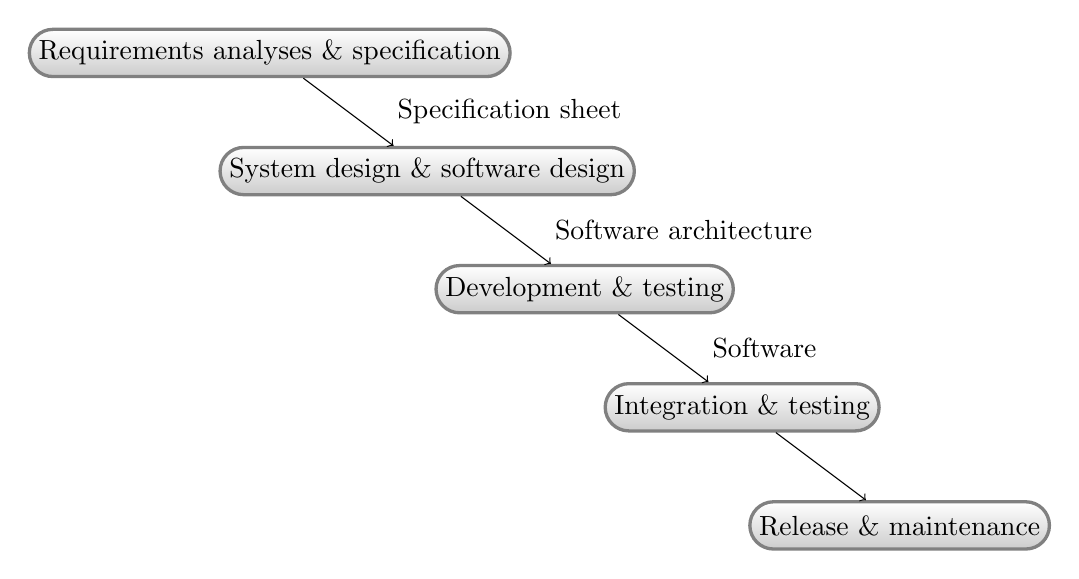
\begin{tikzpicture}[main/.style={
	node distance=10cm,
	rectangle, minimum size=6mm, rounded corners=3mm,
	very thick, draw=black!50,
	top color=white, bottom color=black!20}, node distance=10cm]
	\node[main] (0) {Requirements analyses \& specification};
	\node[main, xshift=2cm, yshift=-1.5cm] (1) {System design \& software design};
	\node[main, xshift=4cm, yshift=-3cm] (2) {Development \& testing};
	\node[main, xshift=6cm, yshift=-4.5cm] (3) {Integration \& testing};
	\node[main, xshift=8cm, yshift=-6cm] (4) {Release \& maintenance};
	\draw[->]
				(0) edge node[midway, right, xshift=0.5cm] {Specification sheet} (1)
				(1) edge node[midway, right, xshift=0.5cm] {Software architecture} (2)
				(2) edge node[midway, right, xshift=0.5cm] {Software} (3)
				(3) edge (4);
\end{tikzpicture} 	
\end{table}
$\bold{Requirements analyses}$ \& $\bold{specification}$: Projektmanagement beginnt, Probleme und Spezifikationen werden zusammengestellt, Anforderungen definiert und dokumentiert \newline
$\bold{System}$ \& $\bold{software design}$: Entwürfe, Modelle und die Softwarearchitektur werden entwickelt \newline
$\bold{Development}$ \& $\bold{testing}$: Software entwickeln und durch Unit-Tests verifizieren \newline
$\bold{integration}$ \& $\bold{system tests}$: Software Komponenten kombinieren und das Gesamtsystem testen \newline
$\bold{Release}$ \& $\bold{maintenance}$: System installieren, Fehler korrigieren, Software an Altern hindern, neue Anforderungen bearbeiten 
\begin{multicols}{2}
$\bold{Pros}$:
\begin{itemize}
	\item Linearer Prozess
	\item Intuitiv
	\item Einfach verständlich
	\item Top-Down
	\item Planbar
	\item Nicht-Unterbrechbar
\end{itemize}
\columnbreak
$\bold{Cons}$:
\begin{itemize}
	\item Feste Phasen
	\item Frühe Festlegung
	\item Keine Wiederholung
	\item Kein Einbeziehen neuer Anforderungen
	\item Oft unpraktisch
\end{itemize}
\end{multicols}
\subsubsection{Iterative Waterfall model}
\begin{table}[H]
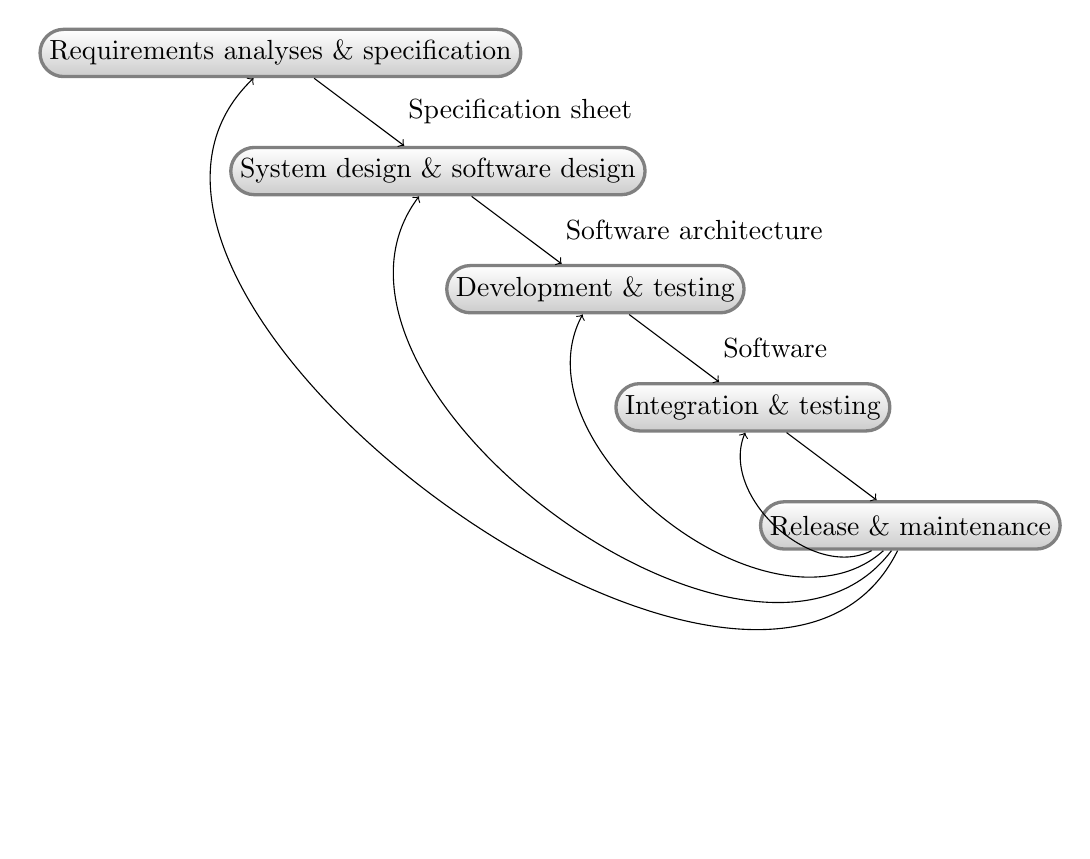
\begin{tikzpicture}[main/.style={
	node distance=10cm,
	rectangle, minimum size=6mm, rounded corners=3mm,
	very thick, draw=black!50,
	top color=white, bottom color=black!20}, node distance=10cm]
	\node[main] (0) {Requirements analyses \& specification};
	\node[main, xshift=2cm, yshift=-1.5cm] (1) {System design \& software design};
	\node[main, xshift=4cm, yshift=-3cm] (2) {Development \& testing};
	\node[main, xshift=6cm, yshift=-4.5cm] (3) {Integration \& testing};
	\node[main, xshift=8cm, yshift=-6cm] (4) {Release \& maintenance};
	\draw[->]
				(0) edge node[midway, right, xshift=0.5cm] {Specification sheet} (1)
				(1) edge node[midway, right, xshift=0.5cm] {Software architecture} (2)
				(2) edge node[midway, right, xshift=0.5cm] {Software} (3)
				(3) edge (4)
				(4) edge [bend left=100] (0)
				(4) edge [bend left=90] (1)
				(4) edge [bend left=80] (2)
				(4) edge [bend left=70] (3);
\end{tikzpicture} 	
\end{table}
\subsubsection{Incremental Waterfall model}
\begin{table}[H]
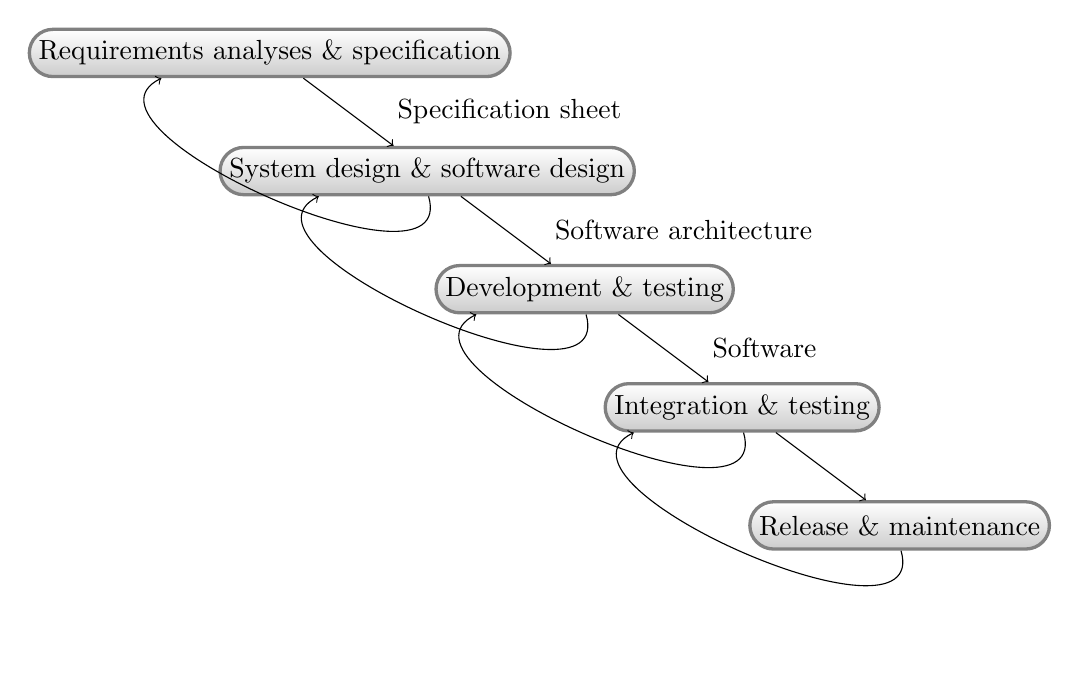
\begin{tikzpicture}[main/.style={
	node distance=10cm,
	rectangle, minimum size=6mm, rounded corners=3mm,
	very thick, draw=black!50,
	top color=white, bottom color=black!20}, node distance=10cm]
	\node[main] (0) {Requirements analyses \& specification};
	\node[main, xshift=2cm, yshift=-1.5cm] (1) {System design \& software design};
	\node[main, xshift=4cm, yshift=-3cm] (2) {Development \& testing};
	\node[main, xshift=6cm, yshift=-4.5cm] (3) {Integration \& testing};
	\node[main, xshift=8cm, yshift=-6cm] (4) {Release \& maintenance};
	\draw[->]
				(0) edge node[midway, right, xshift=0.5cm] {Specification sheet} (1)
				(1) edge node[midway, right, xshift=0.5cm] {Software architecture} (2)
				(2) edge node[midway, right, xshift=0.5cm] {Software} (3)
				(3) edge (4)
				(4) edge [bend left=130] (3)
				(3) edge [bend left=130] (2)
				(2) edge [bend left=130] (1)
				(1) edge [bend left=130] (0);
\end{tikzpicture} 	
\end{table}
\begin{multicols}{2}
$\bold{Pros}$:
\begin{itemize}
	\item Linearer Prozess
	\item Intuitiv
	\item Einfach zu Verstehen
	\item Top-Down
	\item Planbar
	\item Nicht-Unterbrechbar
	\item Wiederholbar
\end{itemize}
\columnbreak
$\bold{Cons}$:
\begin{itemize}
	\item Gefixte Phasen
	\item Frühe Festlegung, aber neue Anforderungen können integriert werden
	\item Veränderte Anforderungen können zu hohen Kosten führen
	\item Struktur tendiert abzubauen
\end{itemize}
\end{multicols}








